\documentclass[../main.tex]{subfiles}


\begin{document}

\section{Evaluation}

In the process of finding test data, there is a benchmark of Detection of Software Clones: {\color{blue} \url{http://www.bauhaus-stuttgart.de/clones/}}. It is a general repository and information center for Detection of Software Clones, it accepts files with labeled clones for clone detection tool evaluation. However its format does not meet our requirement, so again we use manual selection to find ``ground truth'' for testing, just as we did in finding training data: using a low threshold to rule out most of the pairs and manually compare the rest.

We select test data from SWT--since machine learning is based on SWT files. The 10 files we used for testing are: \textit{Button.java, CoolBar.java, Menu.java, Spinner.java, TabFolder.java, TableItem.java, ToolBar.java, ToolItem.java, Tracker.java, Tree.java}. The number of methods ranges from 38 to 147.

Since we have our tool and test data, we are ready to do evaluation. Table \ref{tab:Table_2} shows the test result: \\

\begin{tablehere}
%\small
\begin{tabular}[h]{|c|c|c|c|}
\hline
Test Files & \begin{tabular}{c}TP + FN \\ (Actual \\ Clones) \end{tabular} 
				& \begin{tabular}{c}TP + FP \\ (Detected \\ Clones) \end{tabular} & TP \\
\hline
Button.java & 0 & 4 & 0 \\
\hline
CoolBar.java & 11 & 12 & 10\\
\hline
Menu.java &1 & 0 & 0\\
\hline
Spinner.java & 2 & 2 & 2\\
\hline
TabFolder.java & 3 & 2 & 2 \\
\hline
TableItem.java & 20 & 20 & 18\\
\hline
ToolBar.java & 4 & 4 & 4 \\
\hline
ToolItem.java & 3 & 3 & 3 \\
\hline
Tracker.java & 1 & 1 & 1 \\
\hline
Tree.java & 11 & 13 & 9\\
\hline
\end{tabular}\\
\caption{Test Result}\label{tab:Table_2}
\end{tablehere}

\begin{figurehere}
\centering 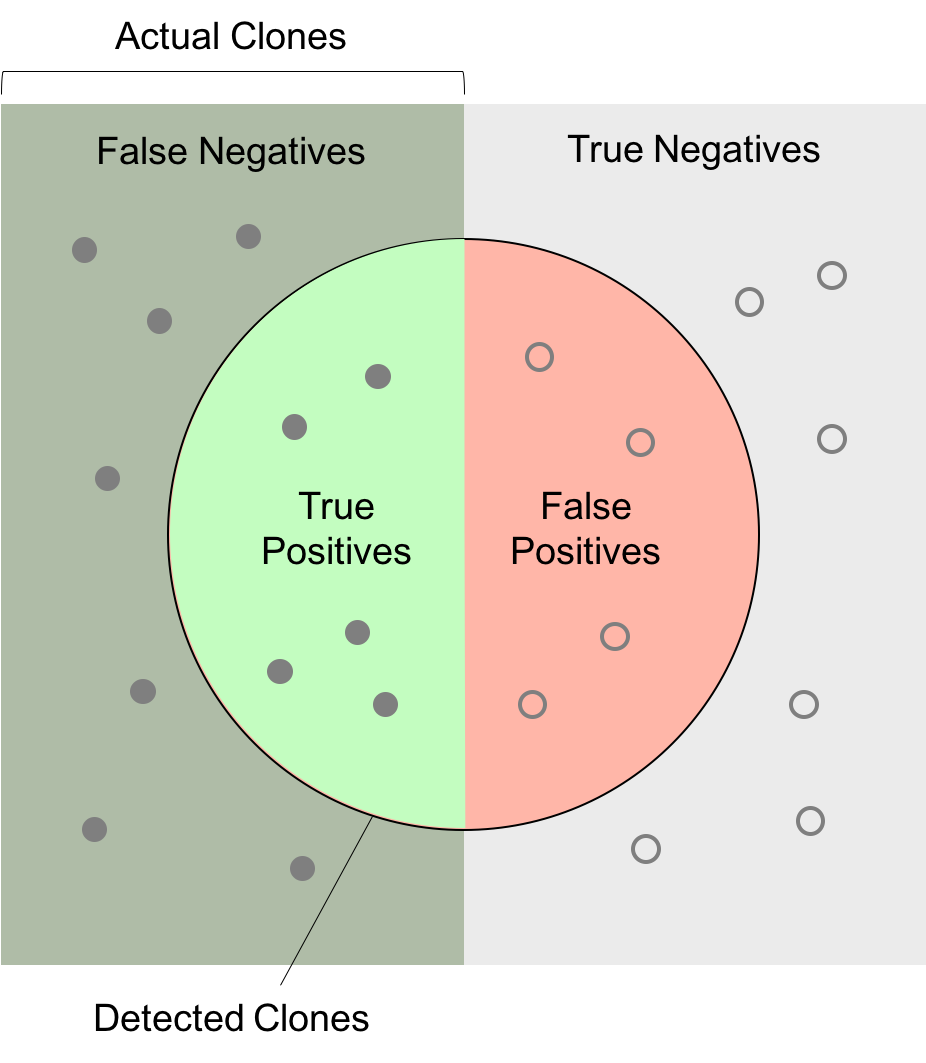
\includegraphics[width = 0.4 \textwidth]{Graph_4} 
\caption{Calculation of Precision and Recall} \label{fig:Graph_4}
\end{figurehere}

From Fig:\ref{fig:Graph_4}, based on the definition of Precision and Recall, 

\begin{equation}
\text{Precision} = \frac{ \text{True Positives}} {\text{Detected Clones}} = \frac{ \text{TP}} {\text{TP} + \text{FP}}
\end{equation}

\begin{equation}
\text{Recall} = \frac{ \text{True Positives}} {\text{Actual Clones}} = \frac{ \text{TP}} {\text{TP} + \text{FN}}
\end{equation}

we are able to evaluate our tool, the precision and recall is given in Fig:\ref{fig:Graph_5}.

\begin{figurehere}
\centering 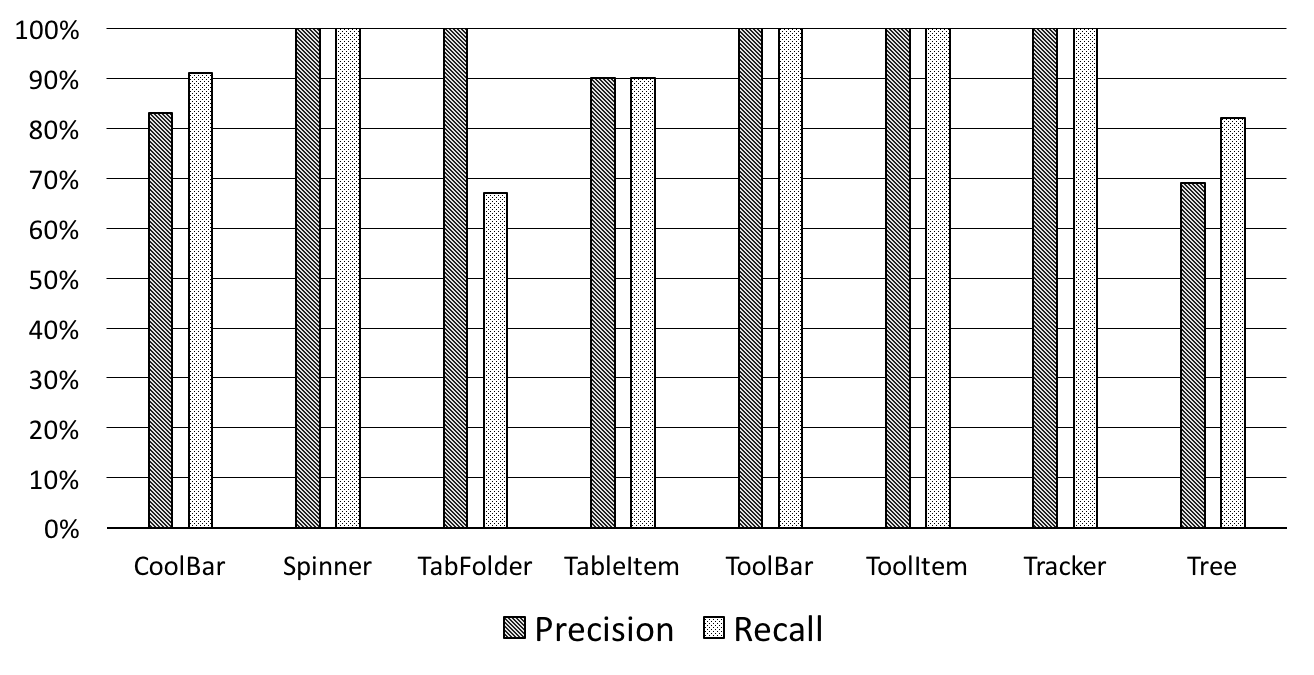
\includegraphics[width = 0.45 \textwidth]{Graph_5} 
\caption{Precision and Recall of STCD} \label{fig:Graph_5}
\end{figurehere}

The time cost of STCD is also evaluated, and is given in Fig:\ref{fig:Graph_6}. Since the comparasion for n methods is $\frac{n(n-1)}{2}$, we expect the time cost to be quadratic, and it turns out to be so--with some variations, which is the result of different method lengths.

\begin{figurehere}
\centering 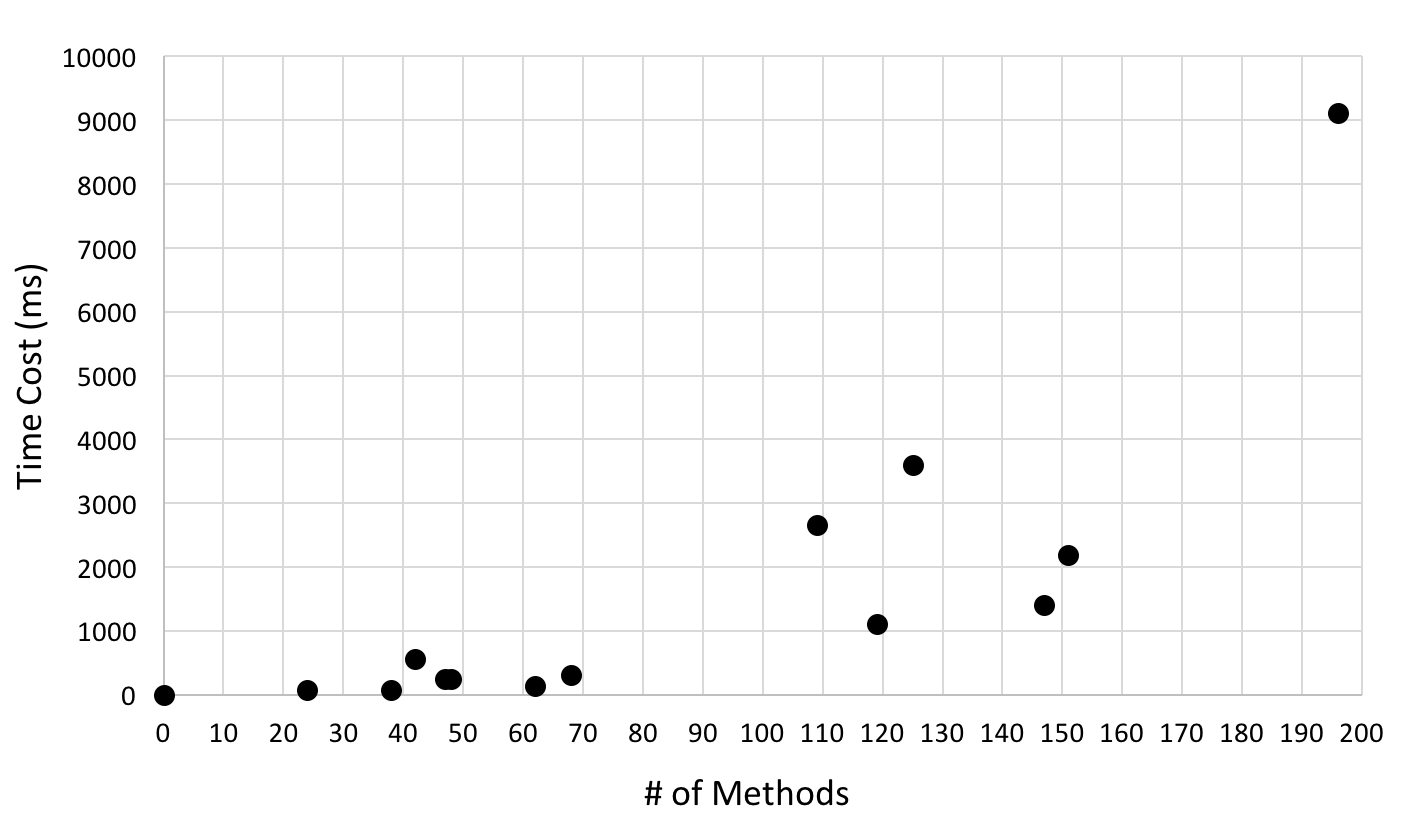
\includegraphics[width = 0.45 \textwidth]{Graph_6} 
\caption{Time Cost of STCD} \label{fig:Graph_6}
\end{figurehere}

\end{document}